\documentclass[11pt]{article}
\usepackage[a4paper,margin=2.4cm]{geometry}
\usepackage{booktabs,graphicx,amsmath,hyperref,xcolor}
\hypersetup{colorlinks,linkcolor=blue!50!black,citecolor=blue!50!black,urlcolor=blue!50!black}
\usepackage[numbers,sort&compress]{natbib}

\title{A One-Way Ratchet:\\
\large Seven Years of Change in AWS Managed IAM Policies}
\author{Mithil Nagabathula\\University of East London\\\texttt{mithilnishu2000@gmail.com}}
\date{October 2026}

\begin{document}
\maketitle
\sloppy

\begin{abstract}
AWS managed policies are permission sets written and maintained by AWS and attached by customers to their own users and roles. When AWS
edits one, every attachment changes at once, without action by the customer. We analyse the public archive that has recorded every
change to every managed policy daily since February 2019: 1{,}669 policies and 11{,}107 recorded modifications. The number of policies
grew from 515 in June 2019 to 1{,}667 in October 2026, and the actions they list grew 6.6-fold, from 9{,}923 to 65{,}873. Of the 2{,}992
modifications that changed which actions a policy grants, 91\% only added actions, 6\% added and removed, and 3\% only removed:
28{,}632 action grants were added against 1{,}796 removed. Policies that existed in 2020 doubled in size; 43\% grew and 1\% shrank.
Modifications that made a statement apply to all resources outnumbered those that scoped one down by 13 to 1, even as the share of
statements on all resources fell from 69\% to 48\% because new policies are scoped better. A small, stable set of 24 policies grants
privilege-escalation actions unconditionally, including two job-function policies; one administrator policy acquired six such actions
in three updates in 2021. A 2026 policy grants every action on every resource, constrained only by a new condition key for actions taken
through an AI-agent interface. For customers, attaching an AWS managed policy is a standing delegation of future permissions to AWS.
\end{abstract}

\section{Introduction}
Least privilege is the oldest principle of access control \cite{saltzer1975}. In AWS, customers can write their own policies or attach
policies that AWS writes and maintains \cite{awsmanaged}. Managed policies are convenient and widely used, but they move a decision out
of the customer's hands: when AWS updates a managed policy, every user and role it is attached to receives the change immediately.
Changes are usually additions needed to support new features, but a principal's effective permissions can grow without any change by
the customer, and without review.

How often does this happen, in which direction, and with what security significance? Automated reasoning over AWS policies is mature
\cite{backes2018zelkova,bouchet2020blockpublic}, but it checks a policy at a point in time. We look at the trajectory. The
MAMIP/IAMTrail project \cite{mamip} has committed the default version of every managed policy to a public Git repository daily since
February 2019, which makes a longitudinal study possible.

\section{Data and method}
\paragraph{Archive.} We cloned the archive in October 2026: 8{,}164 commits, 1{,}669 policies, 11{,}107 recorded modifications. Each
policy file holds the default policy version. A metadata file gives each current policy's path, which distinguishes service-linked
role policies (\texttt{/aws-service-role/}), service-role policies, job-function policies and others; policies no longer listed are
deprecated but kept in the archive.

\paragraph{Snapshots.} For 1 June of each year from 2019 to 2026, and for October 2026, we parsed every policy and counted the action
patterns in its Allow statements, whole-service wildcards (e.g.\ \texttt{s3:*}), partial wildcards (e.g.\ \texttt{s3:Get*}), Allow
statements whose resource is \texttt{*}, and unconditional grants of privilege-escalation actions.

\paragraph{Changes.} For every modification we compared the set of action patterns in Allow statements before and after, and classified
it as an expansion (patterns added only), a contraction (removed only), both, or neutral (no change in action patterns, for example
resource, condition, formatting or metadata changes). Pattern sets are compared syntactically, so replacing \texttt{s3:GetObject} with
\texttt{s3:Get*} counts as one addition and one removal.

\paragraph{Privilege escalation.} We used the action list behind the IAM privilege-escalation methods catalogued by Gietzen
\cite{gietzen2018} (for example \texttt{iam:CreatePolicyVersion}, \texttt{iam:AttachRolePolicy}, \texttt{iam:PassRole},
\texttt{lambda:UpdateFunctionCode}) and counted a policy if an Allow statement matches one of these actions, including through wildcards,
on resource \texttt{*} with no condition. This is a conservative screen: grants scoped to resources or conditions are not counted, and
escalation usually needs a combination of permissions.

\section{Results}
\begin{table}[t]
\centering
\caption{AWS managed policies on 1 June each year and in October 2026: count, actions listed in Allow statements (total, median and 95th percentile per policy), policies using a whole-service wildcard such as \texttt{s3:*}, and the share of Allow statements whose resource is \texttt{*}.}
\label{tab:snap}
\small
\setlength{\tabcolsep}{3.5pt}
\begin{tabular}{lrrrrrr}
\toprule
Snapshot & Policies & Actions listed & Median & 95th pct. & Service wildcard & Allow stmts on \texttt{*} \\
\midrule
2019 & 515 & 9,923 & 7 & 62 & 164 & 69\% \\
2020 & 676 & 13,458 & 7 & 61 & 197 & 66\% \\
2021 & 865 & 18,538 & 8 & 67 & 239 & 62\% \\
2022 & 991 & 23,432 & 8 & 70 & 262 & 58\% \\
2023 & 1140 & 28,881 & 8 & 75 & 281 & 55\% \\
2024 & 1257 & 35,195 & 9 & 78 & 296 & 53\% \\
2025 & 1414 & 44,319 & 10 & 85 & 306 & 50\% \\
2026 & 1568 & 53,139 & 10 & 88 & 322 & 49\% \\
Oct 2026 & 1667 & 65,873 & 10 & 98 & 326 & 48\% \\
\bottomrule
\end{tabular}
\end{table}


\paragraph{Growth.} Table~\ref{tab:snap} and Figure~\ref{fig:growth} show steady growth: about 150 new policies a year since 2020 and a
6.6-fold increase in listed actions since 2019, faster than the 3.2-fold increase in policies, so policies also got larger (median 7 to
10 actions, 95th percentile 62 to 98). Whole-service wildcards appeared in 326 policies, twice as many as in 2019.

\begin{figure}[t]
  \centering
  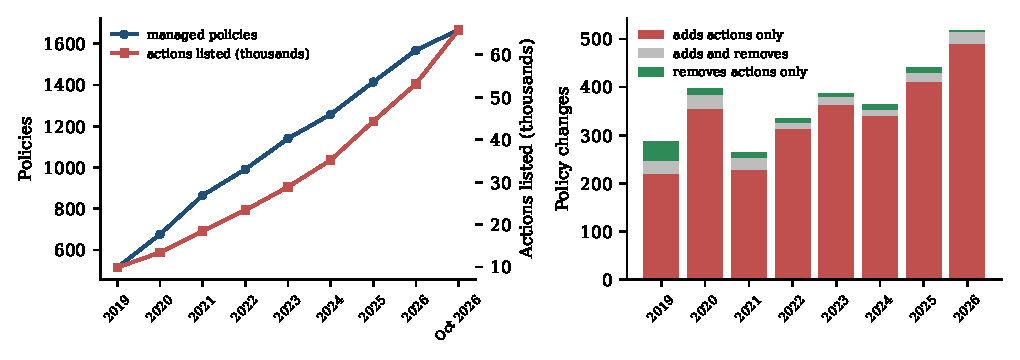
\includegraphics[width=\linewidth]{figures/growth.pdf}
  \caption{Left: managed policies and actions listed. Right: modifications that changed which actions a policy grants, by year and
  direction (neutral changes excluded).}
  \label{fig:growth}
\end{figure}

\paragraph{A one-way ratchet.} Of 11{,}107 modifications, 2{,}992 changed the action patterns a policy grants. Of those, 2{,}723 (91\%)
only added patterns, 168 (6\%) added and removed, and 101 (3\%) only removed. Across all modifications, 28{,}632 patterns were added and
1{,}796 removed. The cohort of 675 policies that existed in June 2020 and still exist grew from 13{,}381 to 26{,}539 listed actions; 43\%
of them grew and 1\% shrank. The largest growth was in broad read-only policies such as \texttt{ReadOnlyAccess}, \texttt{ViewOnlyAccess}
and \texttt{SecurityAudit}, which enumerate new read actions as services launch, so a principal that was ``read-only'' in 2020 can read
far more in 2026.

\paragraph{Resource scope.} The share of Allow statements on all resources fell from 69\% to 48\%, because recently created policies
are scoped more carefully. Changes to existing policies went the other way: 756 modifications increased the number of statements on
\texttt{*} and 58 decreased it.

\paragraph{Privilege escalation.} The number of policies granting a listed escalation action unconditionally on all resources was small
and stable: 24 in 2019 and 24 in 2026. Besides the expected administrator and IAM policies, the set includes the \texttt{DataScientist}
and \texttt{SystemAdministrator} job-function policies, which grant \texttt{lambda:UpdateFunctionCode} on all functions, enough to run
code as any Lambda function's execution role. Only four modifications added escalation actions to an existing policy; three of them were
to \texttt{AdministratorAccess-Amplify} in 2021, which acquired \texttt{iam:AttachRolePolicy}, \texttt{iam:PutRolePolicy},
\texttt{iam:CreatePolicyVersion}, \texttt{iam:PassRole}, \texttt{iam:UpdateAssumeRolePolicy} and \texttt{lambda:UpdateFunctionCode} on
all resources in three steps. Customers who attached it for Amplify development gained the ability to escalate to administrator.

\paragraph{A new pattern: conditional full wildcard.} \texttt{AWSMcpServiceActionsFullAccess}, created in November 2025 and updated in
February 2026, allows every action on every resource when the request carries the condition key \texttt{aws:IsMcpServiceAction}. It is
one of only two current policies whose action is \texttt{*}. Its safety rests entirely on the semantics and enforcement of a single,
new condition key tied to actions taken through an AI-agent tool interface \cite{mcp2024}.

\section{Discussion}
Managed policies trade control for convenience, and the trade grows over time. The direction of change is overwhelmingly towards more
permission, which is unsurprising for policies that must keep up with new features, but it means that attaching a managed policy
delegates future permission decisions to AWS. Customer-side tooling that reviews permissions at attachment time does not see later
growth.

\paragraph{Recommendations.} (1) Treat managed-policy updates as permission changes: subscribe to a change feed (the archive offers
one) and review updates to policies attached in production. (2) Prefer customer-managed copies for sensitive principals, accepting the
maintenance cost. (3) Check job-function policies for escalation paths before using them as defaults. (4) Scrutinise conditional
wildcards such as the MCP policy: a condition key is a single point of failure.

\paragraph{Limitations.} The archive records default versions only, from February 2019, and its early months were built incrementally,
so 2019 figures under-count. Pattern-level comparison does not expand wildcards against the action catalogue, so it understates growth
through wildcards (a fixed \texttt{s3:*} grants every new S3 action) and overstates churn when explicit lists are replaced by wildcards.
The escalation screen ignores scoped and conditional grants and combinations. We do not know how often each policy is attached.

\section{Conclusion}
Over seven years, changes to AWS managed policies almost always added permissions: 91\% of substantive modifications only added, and
grants added outnumbered grants removed sixteen to one. Customers should treat attached managed policies as permissions that change
under them.

\paragraph{Reproducibility.} Analysis code and results will be released at
\newline\url{https://github.com/mithil2k2000-tech/aws-managed-policy-drift}; the archive is public \cite{mamip}.

\paragraph{Use of AI tools.} An AI assistant (Claude, Anthropic) helped write analysis code and draft text. The author designed the
study, reviewed the code and results, and takes responsibility for the content.

\bibliographystyle{plainnat}
\bibliography{refs}
\end{document}
